\ifx\PREAMBLE\undefined
\documentclass{report}
\usepackage[format = hang, font = bf]{caption}
\usepackage{graphicx}
\usepackage{array}
\usepackage{amsmath}
\usepackage{mathtools}
\usepackage{boxedminipage}
\usepackage{listings}
\usepackage{makecell}%diagonal line in table
\usepackage{float}%allowing forceful figure[H]
\usepackage{xcolor}
\usepackage{amsfonts}%allowing \mathbb{R}
\usepackage{alltt}
\usepackage{algorithmicx}
\usepackage[chapter]{algorithm} 
%chapter option ensures that algorithms are numbered within each chapter rather than in the whole article
\usepackage[noend]{algpseudocode} %If end if, end procdeure, etc is expected to appear, remove the noend option
\usepackage{xspace}
\usepackage{color}
\usepackage{url}
\def\UrlBreaks{\do\A\do\B\do\C\do\D\do\E\do\F\do\G\do\H\do\I\do\J\do\K\do\L\do\M\do\N\do\O\do\P\do\Q\do\R\do\S\do\T\do\U\do\V\do\W\do\X\do\Y\do\Z\do\[\do\\\do\]\do\^\do\_\do\`\do\a\do\b\do\c\do\d\do\e\do\f\do\g\do\h\do\i\do\j\do\k\do\l\do\m\do\n\do\o\do\p\do\q\do\r\do\s\do\t\do\u\do\v\do\w\do\x\do\y\do\z\do\0\do\1\do\2\do\3\do\4\do\5\do\6\do\7\do\8\do\9\do\.\do\@\do\\\do\/\do\!\do\_\do\|\do\;\do\>\do\]\do\)\do\,\do\?\do\'\do+\do\=\do\#\do\-}
\usepackage[breaklinks = true]{hyperref}
\lstset{language = c++, breaklines = true, tabsize = 2, numbers = left, extendedchars = false, basicstyle = {\ttfamily \footnotesize}, keywordstyle=\color{blue!70}, commentstyle=\color{red!70}, frame=shadowbox, rulesepcolor=\color{red!20!green!20!blue!20}, numberstyle={\color[RGB]{0,192,192}}}
\mathchardef\myhyphen="2D
% switch-case environment definitions
\algblock{switch}{endswitch} 
\algblock{case}{endcase}
%\algrenewtext{endswitch}{\textbf{end switch}} %If end switch is expected to appear, uncomment this line.
\algtext*{endswitch} % Make end switch disappear
\algtext*{endcase}
\begin{document}
\fi
\chapter{Lexical Analysis}
An implementation of lexical analyzer must do two things:
\begin{enumerate}
\item Recognize substrings corresponding to tokens, i.e. the lexemes.
\item Identify the token class of each lexeme. A token is the $<$token class, lexeme$>$ pair.
\end{enumerate} 
The goal of lexical analysis is to partition the string. It is implemented by reading left-to-right, recognizing one token at a time. ``Lookahead'' might be required to decide where one token ends and the next token begins.
\section{Tools: regular expression and finite automata}
\subsection{Lexical specification \& regular expression}
\begin{enumerate}
\item Write a regular expression for the lexemes of each token class.
\begin{itemize}
\item Number = digit+
\item Keyword = `if' + `else' + $\dots$
\item Identifier = letter (letter + digit)*
\item Openpar = `('
\item $\dots$
\end{itemize}
\item Construct $R$, matching all lexemes of all token classes.

$R$ = Keyword + Identifier + Number + $\dots$ = $R_1 + R_2 + \dots$
\item Let input be $x_1x_2\dots x_n$. For $1\le i\le n$, check if $x_1\dots x_i\in L(R)$.\label{checkinput}
\item If yes, then we know that $x_1\dots x_i\in L(R_j)$ for some $j$.
\item Remove $x_1\dots x_i$ from input and go to \ref{checkinput}.
\end{enumerate}
Problems \& ambiguities:
\begin{enumerate}
\item How much input is used? What if we have 
\begin{equation*}
\begin{split}
x_1\dots x_i&\in L(R)\\
x_1\dots x_j&\in L(R)(i\ne j)
\end{split}
\end{equation*}
at the same time? 

The answer is to choose the {\bf maximal match}: match as long as possible.
\item Which token should be used if more than one token is matched, i.e. what if $x_1\dots x_i$ simultaneously belongs to $L(R_j)$ and $L(R_k)$? 

A priority rule is set up to prevent such ambiguity. Typically, the rule is to {\bf choose the one listed first}. For example, {\sf if} should not be recognized as identifier because it belongs to the language of keyword.
\item What if no rule matches, i.e. what if $x_1\dots x_i\notin L(R)$? This concerns the error handling of the compiler.

The solution is not to let this happen. We will define one more class, the error class, that matches all strings not in the lexical specification, and put it last in priority.
\end{enumerate}
\subsection{Finite automata}
Regex is the specification language of lexical analysis, and finite automata is an implementation mechanism of regex.

A finite automaton consists of
\begin{itemize}
\item An input alphabet $\Sigma$
\item A set of states $S$
\item A start state $n$
\item A set of accepting states $F\subseteq S$
\item A set of transitions $\text{state1}\xrightarrow{\text{input}}\text{state2}$
\end{itemize}
Transition $s_1\xrightarrow{a}s_2$ is read ``in state $s_1$ on input $a$ go to state $s_2$''. If the automaton is in accepting state at the end of the input, it will {\bf accept} the string, meaning that the string is in the language of this machine. Otherwise it will {\bf reject} the string. This is either because it terminates in state $s\notin F$, or because the machine gets stuck: there is no transition defined for the current state and input.

The language of a FA is equal to the set of its accepted strings.

It is possible that the machine changes its state without an input, when the transition is called an $\varepsilon $-move. Depending on whether $\varepsilon$-move is allowed, FA can be classified into two types. {\bf Deterministic Finite Automata (DFA)} make one transition per input and per state, which means for a certain state, an input can lead to at most one possible transition. No $\varepsilon$-move is allowed. {\bf Nondeterministic Finite Automata} can have multiple transitions for one input at a given state, and can have $\varepsilon$-moves.

A DFA takes only one path through the state graph per input string, while an NFA can choose different paths. As long as some of the paths lead to accepting state, the NFA accept the input string.

DFAs and NFAs recognize the same set of languages, which is the set of regular languages. DFAs are faster to execute, while NFAs are in general much (exponentially) smaller.
\section{Implementation}
\begin{figure}[ht]
\centering
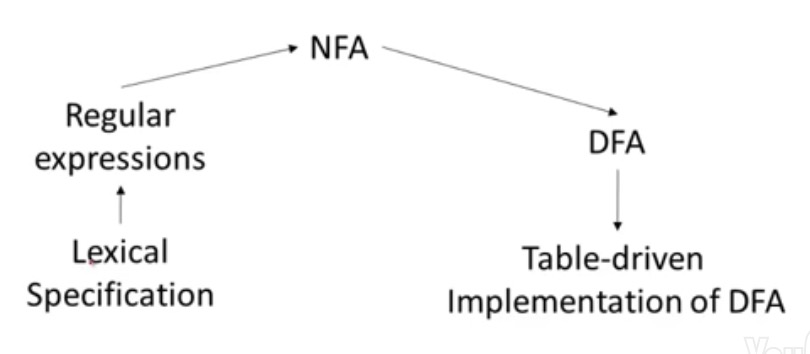
\includegraphics[width = 0.6\textwidth]{LApipeline.jpg}
\caption{Pipeline of lexical analyser}\label{pipeline}
\end{figure}
We will follow the pipeline shown in Figure \ref{pipeline} to implement the lexical analyser step by step.
\subsection{Regular expression into NFAs}
Regex can be transformed into NFAs according to the following rules.

For the simplest $\varepsilon$ regex:
\begin{figure}[H]
\centering
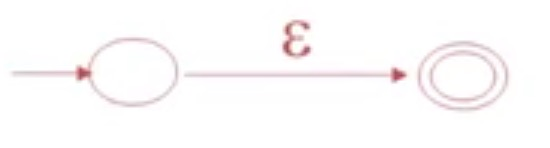
\includegraphics[width=0.3\textwidth]{epsilon.jpg}
\end{figure}
For regex with a single character $a$:
\begin{figure}[H]
\centering
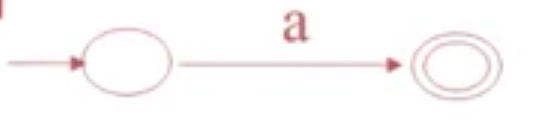
\includegraphics[width=0.3\textwidth]{a.jpg}
\end{figure}
For union $A+B$:
\begin{figure}[H]
\centering
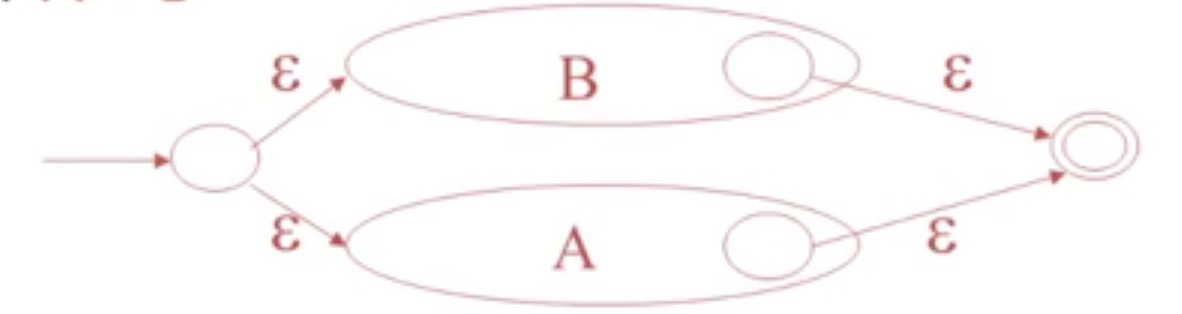
\includegraphics[width=0.5\textwidth]{AplusB.jpg}
\end{figure}
For concatenation $AB$:
\begin{figure}[H]
\centering
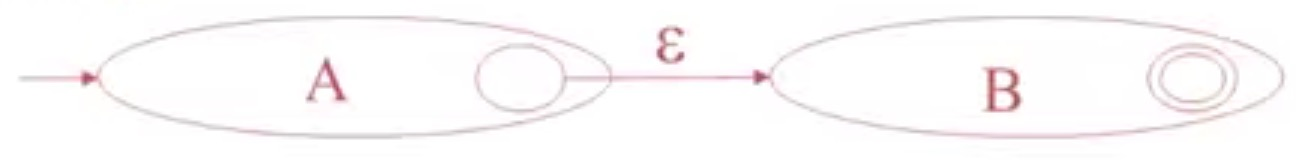
\includegraphics[width=0.5\textwidth]{AB.jpg}
\end{figure}
For iteration $A*$:
\begin{figure}[H]
\centering
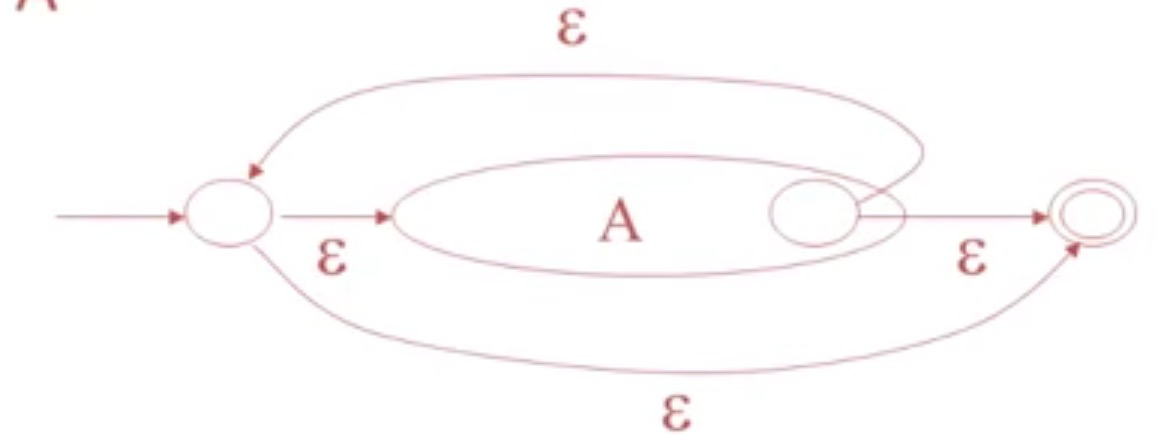
\includegraphics[width=0.5\textwidth]{Astar.jpg}
\end{figure}
By combining the rules above, we can transform any regex into NFAs.
\subsection{NFA to DFA}
We introduce the idea of the {\bf $\varepsilon$-closure} of state. The $\varepsilon$-closure of a state $s$ is the set of the states that can be reached from $s$ following only $\varepsilon$ moves.
\begin{figure}[ht]
\centering
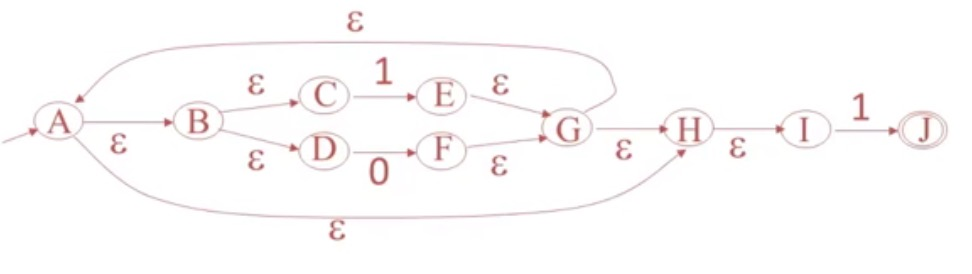
\includegraphics[width = 0.8\textwidth]{nfaeg.jpg}
\caption{Idea of $\varepsilon$-closure}\label{nfaeg}
\end{figure}
In the NFA shown in Figure \ref{nfaeg}, the $\varepsilon$-closure of state $B$ is $\{B,C,D\}$, while the $\varepsilon$-closure of state $G$ is $\{A,B,C,D,G,H,I\}$. We also introduce the denotation $a(X)$, which is defined as 
\begin{equation*}
a(X) = \{y\in S\text{ }|\text{ }\exists x\in X\text{ s.t. }x\xrightarrow{a}y\}.
\end{equation*}

The NFA may be in many different states at any time. Suppose the NFA has $N$ states, and it winds up in a subset of these states $S$. It is for sure that $\lvert S\rvert \le N$. There exist totally $2^N-1$ subsets. $2^N-1$ is a big number, but still a finite one, which means that there exists a way to convert the NFA into a DFA.
\begin{table}[ht]
\centering
\caption{NFA to DFA}\label{nfa2dfa}
\begin{tabular}{c|c|c}
& NFA & DFA \\\hline
states & $S$ & $P(S)-\emptyset$(subsets of $S$ except $\emptyset$)\\
start & $s\in S$ & $\varepsilon\myhyphen clos(s)$\\
final & $F\subseteq S$ & $\{X\in (P(S)-\emptyset)\text{ }|\text{ } X\cap F \neq \emptyset\}$\\
transition &&$X\xrightarrow{a}Y\text{ if }Y = \varepsilon\myhyphen clos(a(X))$\\
\end{tabular}
\end{table}
We set up a series of rules to convert an NFA to a DFA as shown in Table \ref{nfa2dfa}. The state of the DFA records the set of possible states that the NFA could have gotten into with the same input. Below is an example demonstrating this conversion method.
\begin{figure}[H]
\centering
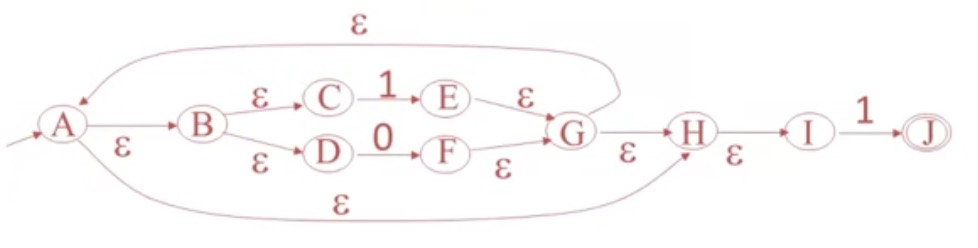
\includegraphics[width=0.8\textwidth]{nfatodfa1.jpg}
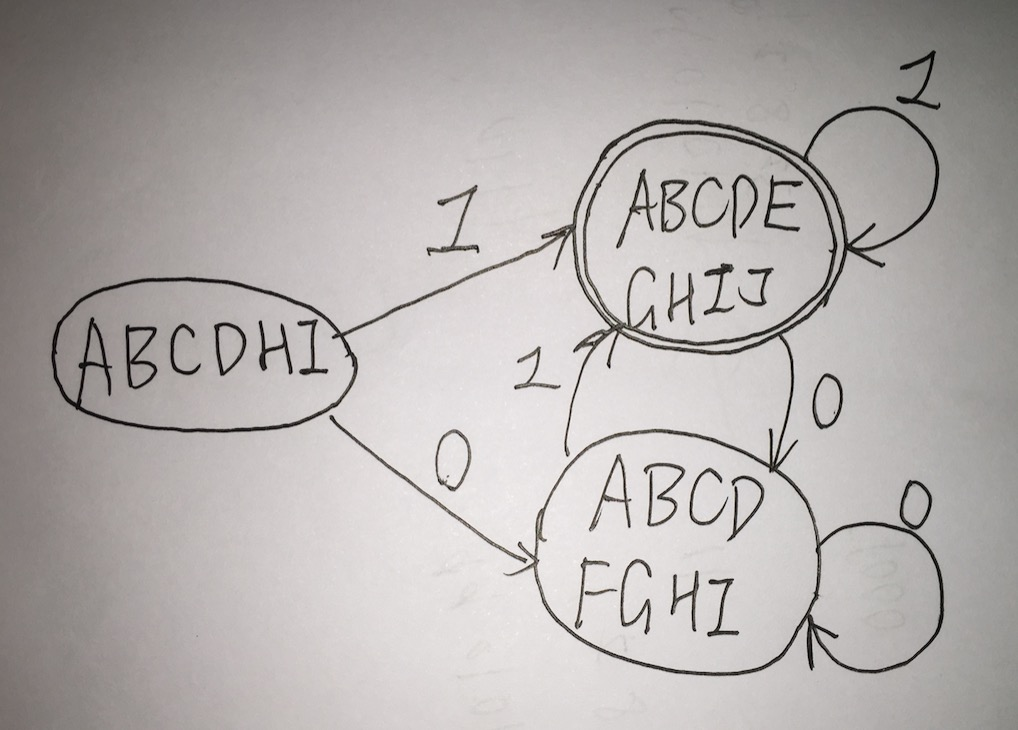
\includegraphics[width=0.5\textwidth]{nfa2dfa2.jpg}
\end{figure}
\subsection{Implementation of FA}
A DFA can be implemented by a 2D {\bf states-input symbol} table $T$. For every transition $s_i\xrightarrow{a}s_k$, there is $T(i,a) = k$. An example is shown below.
\begin{figure}[H]
\centering
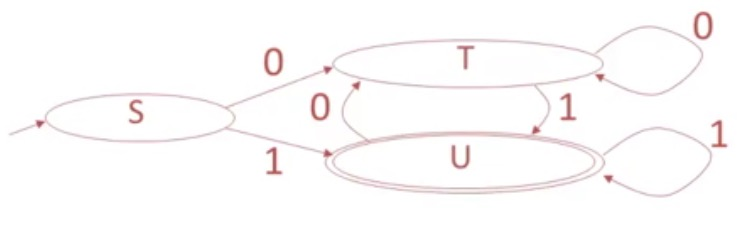
\includegraphics[width=0.6\textwidth]{dfaimpl.jpg}
\end{figure}
\begin{table}[H]
\centering
\begin{tabular}{c|cc}
  & 0 & 1\\\hline
S & T & U\\
T & T & U\\
U & T & U
\end{tabular}
\end{table}
Related C++ code to implement the state update:
\begin{lstlisting}
int i = 0, state = 0;
while (i < len) {
	state = T[state][input[i++]];
} 
\end{lstlisting}
It is also possible to implement the NFA directly without converting it to a DFA, considering that the conversion could be expensive ($N$ states NFA $\rightarrow 2^N-1$ states DFA). It is just a tradeoff between speed and space: DFA is faster but less compact, while NFA is slower but concise.
\ifx\PREAMBLE\undefined
\end{document}
\fi